% Architecture schematic (v2, 2026-10-02). Compile with pdflatex; the page is cropped to the figure.
\documentclass{article}
\usepackage{amsmath,amssymb,bm}
\usepackage{tikz}
\usepackage{graphicx}
\usetikzlibrary{positioning,arrows.meta,fit,backgrounds,calc}
\pagestyle{empty}
\newsavebox\fig
\newcommand{\vcirc}{v_\mathrm{circ}}
\definecolor{feblue}{HTML}{C9DCEE}
\definecolor{feline}{HTML}{1B6CA8}
\definecolor{flyel}{HTML}{F3E2A6}
\definecolor{flline}{HTML}{B8860B}
\definecolor{feinner}{HTML}{E3EEF8}
\definecolor{feinnerline}{HTML}{1B6CA8}
\definecolor{flinner}{HTML}{FBF3D5}
\definecolor{flinnerline}{HTML}{B8860B}
\definecolor{iogrey}{HTML}{F1F1F1}
\definecolor{fib}{HTML}{D1495B}
\begin{document}
\savebox\fig{%
\begin{tikzpicture}[
  font=\small,
  >={Latex[length=2.2mm]},
  box/.style={draw=black!70, rounded corners=2pt, align=center, inner sep=4pt, line width=0.5pt},
  fe/.style={box, fill=feinner, draw=feinnerline, minimum width=2.7cm, minimum height=1.0cm},
  fl/.style={box, fill=flinner, draw=flinnerline, minimum width=3.6cm, minimum height=1.3cm},
  io/.style={box, fill=iogrey, minimum width=2.9cm, minimum height=1.25cm},
  lab/.style={font=\scriptsize, text=black!75},
  arr/.style={->, line width=0.6pt, draw=black!75},
]
% ---------------- inputs ----------------
% image and spectra of Xu3 galaxy 6447 (e_arch_thumbnails.py)
\node[inner sep=0, anchor=south west] (img) at (0,4.4) {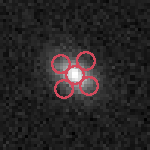
\includegraphics[width=2.0cm]{thumb_image.pdf}};
\draw[black!70] (img.south west) rectangle (img.north east);
\node[lab, above] at (img.north) {Image ($48\times48$)};
\node[inner sep=0, anchor=south west] (spec) at (0,1.75) {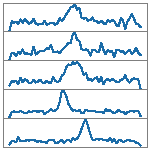
\includegraphics[width=2.0cm]{thumb_spectra.pdf}};
\node[lab, above] at (spec.north) {Fiber spectra ($5\times64$)};
% metadata
\node[io, minimum width=2.0cm, minimum height=1.0cm, font=\scriptsize] (meta) at (1,0.55) {Fiber positions,\\ $m_r$, $\rho_I$, $\rho_S$};
\node[lab, above] at (1,1.05) {Metadata};
\coordinate (imgR) at (2.0,5.4); \coordinate (specR) at (2.0,2.75);
% ---------------- feature extraction ----------------
\node[fe] (cnnI) at (4.55,5.4) {Image CNN\\ \scriptsize (ResNet)};
\node[fe] (cnnS) at (4.55,2.75) {Spectra CNN};
\node[fe] (mlp)  at (4.55,0.55) {Metadata MLP};
\draw[arr] (imgR) -- (cnnI); \draw[arr] (specR) -- (cnnS); \draw[arr] (meta) -- (mlp);
\node[box, fill=feinner, draw=feinnerline, minimum width=1.25cm, minimum height=5.9cm, rotate=0] (cat) at (7.55,3.0) {};
\node[rotate=90, align=center] at (cat) {Concatenate + LayerNorm};
\draw[arr] (cnnI.east) -- node[lab, above]{512} (cnnI.east -| cat.west);
\draw[arr] (cnnS.east) -- node[lab, above]{512} (cnnS.east -| cat.west);
\draw[arr] (mlp.east)  -- node[lab, above]{128} (mlp.east -| cat.west);
\begin{scope}[on background layer]
  \node[draw=feline, fill=feblue, rounded corners=4pt, line width=0.8pt, fit=(cnnI)(mlp)(cat), inner xsep=8pt, inner ysep=10pt, yshift=4pt] (FE) {};
\end{scope}
\node[font=\small\bfseries, text=feline, anchor=south west] at (FE.north west) {Feature extraction};
% ---------------- normalizing flow ----------------
\node[fl] (maf) at (12.73,4.55) {Bounded spline flow\\ \scriptsize (4 masked autoregressive layers)};
\node[lab, below=1pt of maf, align=center] (mafp) {$g_1, g_2, \cos i, v_0, \vcirc$\\$R_\mathrm{vscale}, R_h, \log_{10}F_{\mathrm{H}\alpha}$};
\node[fl] (circ) at (12.73,1.15) {Circular spline flow\\ \scriptsize $\theta_\mathrm{int}$};
\draw[arr] (mafp.south) -- node[lab, right]{conditions on $\mathbf{x}'$} (circ.north);
\coordinate (cin) at (10.15,3.0);
\draw[line width=0.6pt, draw=black!75] (cat.east |- cin) -- (cin);
\node[lab, anchor=south] at (9.15,3.02) {condition};
\node[lab, anchor=north] at (9.15,2.98) {1152};
\draw[arr] (cin) |- (maf.west); \draw[arr] (cin) |- (circ.west);
\node[box, fill=flinner, draw=flinnerline, font=\scriptsize, minimum width=1.3cm, minimum height=0.9cm] (b1) at (16.13,4.55) {$\mathcal{U}[0,1]^8$};
\node[box, fill=flinner, draw=flinnerline, font=\scriptsize, minimum width=1.3cm, minimum height=0.9cm] (b2) at (16.13,1.15) {$\mathcal{U}(-\pi,\pi)$};
\draw[<->, line width=0.6pt, draw=black!75] (maf) -- (b1); \draw[<->, line width=0.6pt, draw=black!75] (circ) -- (b2);
\node[lab, above=0pt of b1] {base};
\node[lab, above=0pt of b2] {base};
\begin{scope}[on background layer]
  \node[draw=flline, fill=flyel, rounded corners=4pt, line width=0.8pt, fit=(maf)(mafp)(circ)(b1)(b2)(cin), inner xsep=8pt, inner ysep=12pt, yshift=2pt] (FL) {};
\end{scope}
\node[font=\small\bfseries, text=flline!90!black, anchor=south west] at (FL.north west) {Posterior estimation};
% ---------------- outputs ----------------
\node[io, anchor=west, font=\scriptsize] (train) at (17.63,4.55) {\textbf{Training}\\[1pt] minimize NLL\\ $-\log q_\psi(\mathbf{x}\mid\mathbf{c})$};
\node[io, anchor=west, font=\scriptsize] (inf) at (17.63,1.15) {\textbf{Inference}\\[1pt] posterior samples\\ $\to$ TF reweighting};
\draw[arr] (FL.east |- train.west) -- (train.west);
\draw[arr] (FL.east |- inf.west) -- (inf.west);
\end{tikzpicture}}
\pdfpagewidth=\wd\fig \pdfpageheight=\dimexpr\ht\fig+\dp\fig\relax
\hoffset=-1in \voffset=-1in \topmargin=0pt \headheight=0pt \headsep=0pt \oddsidemargin=0pt \parindent=0pt \topskip=0pt
\noindent\usebox\fig
\end{document}
